\chapter{10 Questions with a Millionaire: Robert Miller on Cashflow, Brand, and Compounding}

We can read this interview as a lecture on entrepreneurial compounding. The speaker keeps returning to a small set of quantities that either accumulate or decay across time: reputation, acquisition skill, cashflow discipline, partner alignment, learning capital, and health. There is no blackboard here, but there is still a mathematical spine: some states survive a failed venture, some do not, and the difference determines how quickly the next venture can move.

\section{The Asset That Survives the Reset}

The cold open gives the result before the explanation. Two earlier agencies shut down; later businesses moved faster. The reason, as the speaker presents it, is that the personal brand was being built alongside the businesses, so the business shell could reset while the market's memory did not.

As a bookkeeping device, we may gather the main entrepreneurial state variables into
\begin{equation}
X_t=(B_t,K_t,C_t,P_t,H_t),
\end{equation}
where \(B_t\) is personal brand and reputation, \(K_t\) is learned capability, \(C_t\) is operating cashflow, \(P_t\) is partner quality and alignment, and \(H_t\) is health or usable work capacity.

The opening claim is then compressed by
\begin{equation}
\text{Shutdown of venture}_i \not\Rightarrow B_{i+1}=0.
\end{equation}
This is not the speaker's notation; it is a cautious reconstruction of the logic behind the teaser. The point is that the business vehicle may disappear while reputation, audience trust, and accumulated market goodwill continue forward.

That distinction gives us two classes of entrepreneurial objects:
\begin{itemize}
\item durable quantities: reputation, audience trust, learned acquisition skill, judgment,
\item transient quantities: a specific offer, a particular agency structure, a given partner mix, a current traffic channel.
\end{itemize}

The rest of the lecture can be read as an attempt to explain which quantities compound, which quantities reset, and which mistakes destroy the compounding process.

\section{College, Capital Gains, and the Search for a Real Business}

After the formal introduction, Miller describes his path through digital marketing, e-commerce, and crypto, and then immediately turns to the question of college. His answer is not simply anti-college. Rather, he distinguishes between paths that require formal pedigree and paths that reward problem-solving ability more directly.

What sharpens the discussion is the next move. He says that he had already made some money in crypto, but that this was not yet a business. The key distinction is
\begin{equation}
G \neq C,
\end{equation}
where \(G\) denotes capital gains and \(C\) denotes operating cashflow.

That is the decisive transition in the lecture. We may hold an asset that appreciates, and we may even realize substantial gains, but this does not yet solve the entrepreneurial problem. The entrepreneurial problem is to build something that produces recurring inflow rather than one-time appreciation. In his telling, that realization is what made marketing education matter.

\subsection{Question \& Answer}

\paragraph{Question.} Why can college be optional for entrepreneurial work and still remain necessary for other careers?

\paragraph{Answer.} The answer given in the lecture is structural rather than ideological. Some professions rely on formal credentialing and institutional trust. Entrepreneurship, as Miller frames it here, does not begin with pedigree but with problem-solving, market fit, and the ability to generate cashflow. College may help, but it is not the core mechanism. The core mechanism is learning how to create value that a market will pay for repeatedly.

This is why the transition from school to outside coursework matters so much in the lecture. The important move was not merely leaving one educational path for another. The important move was passing from passive exposure to active skill acquisition in a domain that could generate revenue.

\section{Scaling: Marketing, Sales, Then Finance}

When asked how to scale a business, Miller does not offer a loose list. He gives an order. First we bring attention. Then we convert it. Then we understand the money that results. In compact form,
\begin{align}
\text{Traffic} &\to \text{Leads},\\
\text{Leads} &\to \text{Sales},\\
\text{Sales} &\to \text{Revenue}.
\end{align}

He then adds a third term that entrepreneurs often postpone:
\begin{equation}
\text{Scale} \Leftarrow (M \to S \to F),
\end{equation}
with \(M\) for marketing, \(S\) for sales, and \(F\) for finance.

The order matters. Marketing is not merely paid ads; in the lecture it means content and traffic strategy, the work of getting people to care about what is being said or offered. Sales is then the ability to convert attention into paying customers. Finance comes after this because one cannot manage cashflow one has not yet learned to generate.

\begin{figure}[h]
\centering
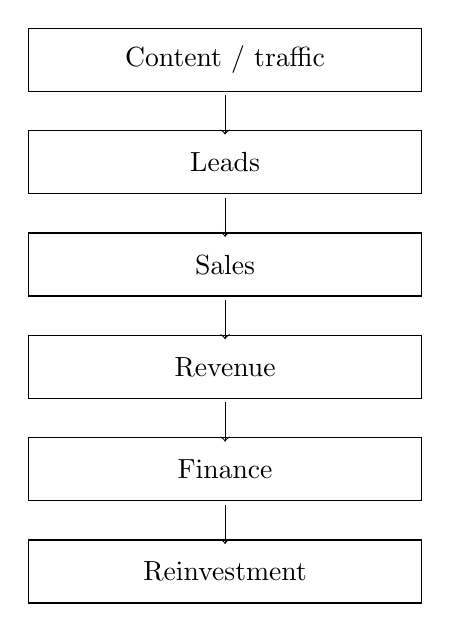
\begin{tikzpicture}[x=1cm,y=1cm]
\draw (0,0) rectangle (5,0.8);
\node at (2.5,0.4) {Content / traffic};

\draw[->] (2.5,-0.05) -- (2.5,-0.55);

\draw (0,-1.3) rectangle (5,-0.5);
\node at (2.5,-0.9) {Leads};

\draw[->] (2.5,-1.35) -- (2.5,-1.85);

\draw (0,-2.6) rectangle (5,-1.8);
\node at (2.5,-2.2) {Sales};

\draw[->] (2.5,-2.65) -- (2.5,-3.15);

\draw (0,-3.9) rectangle (5,-3.1);
\node at (2.5,-3.5) {Revenue};

\draw[->] (2.5,-3.95) -- (2.5,-4.45);

\draw (0,-5.2) rectangle (5,-4.4);
\node at (2.5,-4.8) {Finance};

\draw[->] (2.5,-5.25) -- (2.5,-5.75);

\draw (0,-6.5) rectangle (5,-5.7);
\node at (2.5,-6.1) {Reinvestment};
\end{tikzpicture}
\end{figure}

We may summarize the lecture's ordering principle in a simple causal chain:
\begin{enumerate}
\item Marketing brings attention and traffic.
\item Attention becomes useful only when it creates leads.
\item Sales converts leads into revenue.
\item Finance determines whether revenue becomes stable cashflow.
\item Stable cashflow creates the possibility of reinvestment.
\end{enumerate}

In this sequence, each term prepares the next. The lecture does not let us skip from attention directly to scale.

\section{Strategic Frameworks and the Persistence of Reputation}

The book-recommendation segment is not a side note. It is the lecture's bridge from tactics to strategy. \emph{The Road Less Stupid} is recommended because it trains the entrepreneur in what to think about before acting; \emph{Multipliers} because growth soon becomes a question of other people's output; \emph{Predictable Revenue} because sales must become systematic rather than accidental.

This segment sets up the next move, which is the return to the opening claim about personal brand. Miller argues that the specific mechanism by which a business makes money can change. Offers change, traffic environments change, even the type of company may change. What persists is the accumulated market reputation of the operator.

A cautious way to represent that idea is through a simple update rule:
\begin{equation}
B_{t+1}=B_t+\Delta R_t,
\end{equation}
where \(\Delta R_t\) denotes the reputation earned through repeated market contact, delivery, and visibility.

This is again editorial notation, not a quoted formula. But it captures the claim that the next launch does not begin at zero if the operator's name already carries trust. The function of the personal brand, in this lecture, is not vanity. It is continuity across discontinuous ventures.

\subsection{Question \& Answer}

\paragraph{Question.} What actually carries forward when a company shuts down?

\paragraph{Answer.} The lecture's answer is not the legal shell, not the old offer, and not even necessarily the same team. What carries forward is the operator's accumulated standing in the market: a track record, an audience, and the ability to acquire clients because the market already associates that person with a useful function. The cold open is then no longer mysterious. Repeated shutdowns do not imply repeated zeroes.

\section{Failure, Partnerships, and Incentive Alignment}

Once the lecture has established what can persist individually, it turns to what fails collectively. Miller's answer to failure is diagnostic rather than sentimental. He points to too many partners, ego around ideas, and the tendency to overvalue naming and concept relative to execution.

His rough numerical rule is
\begin{equation}
n_{\text{partners}} \lesssim 3.
\end{equation}
This is plainly experiential rather than theorem-like, but it matters because it treats coordination itself as a real constraint.

The next refinement is qualitative. A partner should not be present merely because he is liked. A partner should bring something structurally necessary to the business. In words drawn from the lecture, the relevant contributions are connections, people, capital, execution, and network. Just as important is value alignment: under stress, shared language about what the business is for and where it is going becomes the test of whether the partnership can survive.

\subsection{Question \& Answer}

\paragraph{Question.} Why was the payroll-support loan a bad financial decision even though it was repaid quickly?

\paragraph{Answer.} The financial loss itself was not the main issue. The repayment, by his account, was manageable. What made the decision bad was informational: it revealed that the burden of risk was not shared. He took liability in order to preserve payroll, and the others did not proportionally underwrite that decision. So the badness of the decision lies not only in the loan but in what the loan exposed about commitment and incentives.

This is a subtle point and worth preserving. A decision can be financially survivable and still be structurally wrong. In the lecture, the loan functions as a stress test for partnership quality.

\section{Cryptocurrency as a Question About Value}

The crypto segment is the lecture's clearest conceptual problem. Miller does not present cryptocurrency merely as a speculative asset class. He presents it as a question about what a society takes to be valuable.

The puzzle may be written in two competing schematic forms:
\begin{align}
V &\stackrel{?}{\propto} \text{scarcity},\\
V &\stackrel{?}{\propto} \text{scarcity}+E,
\end{align}
where \(V\) is perceived value and \(E\) is extraction or verification cost.

He illustrates the second form by analogy. Gold is not valuable merely because it is hard to find; it must also be mined. Bitcoin, in his account, is not only scarce but requires real physical infrastructure and electricity in order to verify transactions. The lecture stops short of a completed theory here. It stages the question and leaves its full resolution open.

\subsection{Question \& Answer}

\paragraph{Question.} Is something valuable because it is scarce, or because scarce value is backed by real cost?

\paragraph{Answer.} The lecture does not force a final answer. It instead sharpens the distinction. Mere rarity is one candidate for value. Scarcity backed by energy expenditure, mining, or verification is another. Miller treats Bitcoin and gold as structurally analogous in this respect. He then adds an additional question: even if such assets can store value, should they mainly be used for transacting, or should they be held and preserved?

The important thing in the notes is to retain the open character of the argument. This is Miller's way of posing the problem, not a settled monetary theorem.

The lecture then narrows from the conceptual question back to biography. Miller describes entering crypto in roughly 2015--2016, hearing about Bitcoin early, seeing wallet sizes and transaction histories large enough to make the scale impossible to ignore, and then entering himself.

\paragraph{Worked example.} The first financial break is described quantitatively. In the lecture,
\begin{align}
I_0 &\approx \$1.5\text{k}-\$2\text{k},\\
V_{4\text{ mo}} &\approx \$250\text{k}.
\end{align}
So the rough multiple is
\begin{align}
m=\frac{V_{4\text{ mo}}}{I_0}
\approx
\begin{cases}
250000/2000 = 125,\\
250000/1500 \approx 166.7.
\end{cases}
\end{align}

The important point is not just the size of the gain. A multiple in this range changes the entrepreneur's feasible action set. It can fund time, attention, experimentation, and education. In Miller's telling it also created a second form of leverage: he could explain the space to others, teach it, and thereby discover that helping people understand something scarce can itself become an entrepreneurial mechanism.

\section{Self-Investment, Health, and the Evolving Why}

The lecture's best financial decision is deliberately paired against the worst one. After making money in crypto, Miller says he invested the rest into courses. In the lecture this is not presented as consumption but as capability formation:
\begin{equation}
I_{\text{education}} \approx \$30\text{k}-\$40\text{k}.
\end{equation}

A cautious reconstruction of the compounding intuition is
\begin{equation}
K_{t+1}=K_t+L_t,
\end{equation}
where \(L_t\) is one learning investment, and
\begin{equation}
R_{t+k}=f\!\left(\sum_{i\le t} L_i\right).
\end{equation}
The point is not that the return comes cleanly from one course or one mastermind. The point is that later revenue may be the visible payoff of many earlier learning inputs, with the final mentorship acting as catalyst rather than sole cause.

\subsection{Question \& Answer}

\paragraph{Question.} Why can the best investment look nonlinear, with the return appearing only after several earlier inputs have accumulated?

\paragraph{Answer.} Because learning compounds unevenly. The lecture is explicit here: one program may appear to generate the breakthrough, but in reality it may only complete a chain that was already being built by earlier study. The final visible jump can therefore be large even though no single input fully explains it. In that sense, self-investment behaves more like a threshold process than a smooth line.

The lecture then broadens further. The next lesson is not about money at all, at least not directly. It is about relationships, health, and motive. One keeps only a small number of people who truly matter; one cannot treat health as an infinite reserve; and one cannot understand the work without understanding the reason for doing it.

The health warning is quantitative enough to deserve a compact summary:
\begin{equation}
t_{\text{work}} \approx 16\,\mathrm{h/day},
\qquad
t_{\text{sleep}} \approx 0
\text{ for } 24\text{--}48\,\mathrm{h}.
\end{equation}
In the lecture this is not heroism. It is a failure mode. The breakdown that followed is the evidence that entrepreneurial effort runs against a hard biological boundary.

The final move is from business to \emph{why}. At first the why is survival and provision; later it becomes something broader, the chase toward potential, impact, and the ability to care for family without repeating the scarcity of childhood. This closing matters because it changes the scale of evaluation. Revenue, brand, and skill are not abandoned. They are subordinated to a more final question: what kind of person is this work allowing one to become, and for whom is the gain being made useful?

\section{Summary}

This interview can be read as a compact theory of entrepreneurial compounding. The first lesson is that not all assets are equally fragile: a venture may fail while reputation survives. The second is that gains are not the same thing as cashflow, and that scaling follows an order from marketing to sales to finance. The third is that teams fail when execution and incentives separate, and that capital allocation into learning can produce delayed but nonlinear returns.

The lecture closes by widening the frame. Relationships, health, and motive are not decorative add-ons to business success. They are the constraints and purposes that determine whether the compounding process remains worth sustaining at all.